\section{Implementation}
\label{s:implementation} % This declares a label so you can reference the section elsewhere.

To understand how address space layout randomization works in Linux, one must first know how an address space is laid out for a particular process. There are three main parts of a process’s address space: text, data, and stack \cite{memorylayout}. The text space holds the executable code of the process. This is a static, read-only block of memory. Next, there is the data segment. This section stores the program’s variables, in particular the primitives, arrays, and strings that the programmer declared. Finally, there is the stack, which is a Last-In-First-Out (LIFO) structure that contains information about the program’s execution subroutines. The text segment is traditionally at the bottom of the address space, followed by the data, with the stack located at the end of the allocated address space. The layout can be seen in Figure \ref{f:memory_layout}.

\begin{figure}
\centering % Make it center
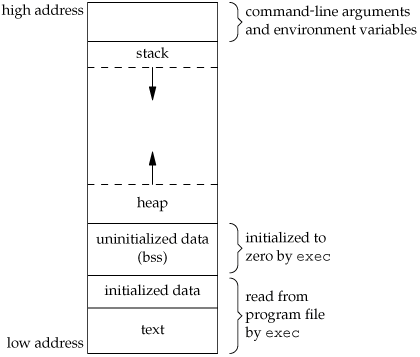
\includegraphics[width=0.5\textwidth]{figures/Memory-Layout.png}
\caption{The layout of a process's memory in Linux \cite{memorylayout}}
\label{f:memory_layout}
\end{figure}

While the predictability of the locations of these parts of the address space would seem convenient, it can assist serious security attacks, such as the one detailed above. ASLR randomizes key parts of the virtual address space for a process. There are differing and weaker variations to this system. Because ASLR can introduce performance penalties on systems with smaller memory sizes, the security benefits may not always outweigh the performance loss. Different operating systems will sometimes only implement ASLR for crucial security components, for example. The level of randomization that occurs can be chosen when compiling the Linux kernel using the randomize\_va\_space sysctl file. There are three main options: 0 for no randomization, 1 for randomization of the mmap base, stack, and VDSO page, and 2 for complete randomization, which includes the heap. \cite{kerneldocs}

In a nonrandomized process, the location of the stack is in the same place on every execution. However, in an operating system with ASLR enabled, a process’s address space is randomized at runtime, and therefore the stack will be in a different place every time the process is created. The kernel acts as a middle-man and keeps track of where the randomized pieces are located. The source for the function in the Linux kernel that is used to randomize the addresses is shown below. It’s main purpose is to “return a start address such that a <range> with size 'len' starting at the return value is inside in the area defined by [start, end], but is otherwise randomized.” \cite{randomc} The result is that the stack is now in an unknown location, significantly reducing the effectiveness of stack buffer overflow attack.

\begin{lstlisting}[caption=Source for the range randomization function]
unsigned long randomize_range(unsigned long start, unsigned long end, unsigned long len)
{
	unsigned long range = end - len - start;

	if (end <= start + len)
		return 0;
	return PAGE_ALIGN(get_random_int() % range + start);
}
\end{lstlisting}
